\clearpage
\section{Appendix}

\subsection{Experimental Details}
\label{appendix:exp_details}
In this section, we provide further details of the experimental setup described in Section~\ref{subsec:setup} and the hyper-parameters used for all the runs in Table~\ref{tab:hp}. For all the tasks, we use a mini-batch \SGD optimizer for local training at the client and \FedAvg optimizer for global model update on the server. The LEAF benchmark is released under the BSD 2-Clause License.

\paragraph{Baselines.} We run hyper-parameter sweeps to tune the client and server learning rates for the uncompressed baselines. Then, we keep the same hyper-parameters in all the runs involving uplink compression. We have observed that tuning the hyper-parameters for each compression factor does not provide significantly different results than using those for the uncompressed baselines, in addition to the high cost of model training involved.

\paragraph{Compression details.}For scalar quantization, we use per-tensor quantization with MinMax observers. We use the symmetric quantization scheme over the integer range $[-2^{b-1}, 2^{b-1} - 1]$. For pruning, we compute the random mask separately for each tensor, ensuring all pruned layers have the same target sparsity in their individual updates. For product quantization, we explore various configurations by choosing the number of codewords per layer $k$ in $\{8, 16, 32, 64\}$ and the block size~$d$ in $\{4, 9, 18\}$. We automatically adapt the block size for each layer to be the largest allowed one that divides $C_{\text{in}}$ (in the fully connected case).

\begin{table}[!ht]
 \caption{Hyper-parameters used for all the experiments including baselines. $\eta$ is the learning rate.}
    \centering
    \begin{tabular}{l|ccccc}
    \toprule
    Dataset & Users per round & Client epochs & Max. server epochs & $\eta_\mathrm{\SGD}$ & $\eta_\mathrm{\FedAvg}$ \\
    \midrule
    CelebA & 100 & 1 & 30 & 0.90 & 0.08 \\
    Sent140 & 100 & 1 & 10 & 5.75 & 0.24 \\
    FEMNIST & 5 & 1 & 5 & 0.01 & 0.24 \\
    \bottomrule
    \end{tabular}
    \label{tab:hp}
\end{table}


\subsection{Experimental Results}
\label{appendix:results}

We provide various additional experimental results that are referred to in the main paper.
\subsubsection{Tables Corresponding to Figure~\ref{fig:results_summary}}
\label{appendix:table}
We provide the detailed results corresponding to Figure~\ref{fig:results_summary} along with standard deviation over 3 runs in Tables~\ref{tab:fig2_sq}, \ref{tab:fig2_prune}, and \ref{tab:fig2_pq}.

\subsubsection{Aggregation overflows with Scalar Quantization}
\label{appendix:overflow}
We discussed the challenge of aggregation overflows of quantized values with restricted \SecAgg finite group size in Section~\ref{subsec:sq} and noted in Section~\ref{subsubsec:sq_sa} that it suffices for \SecAgg bit-width~$p$ to be greater than quantization bit-width $b$ by at most $\lceil\log_2 N\rceil$, where $N$ is the number of clients participating in a given round. However, the overflow margin increases the client update size by~$p - b$ per weight. To optimize this further, we explore the impact of $p$ on aggregation overflows and accuracy, and present the results in Table~\ref{tab:celeba_overflows}.
As expected, we observe a decrease in percentage of weights that overflow during aggregation with the increase in the overflow margin size. However, while there is some benefit to non-zero overflow margin size, there is no strong correlation between the overflow margin size and accuracy, indicating the potential to achieve better utility even in the presence of overflows.

\begin{table}[!ht]
    \caption{Percentage of aggregation overflows (among all model parameters) for the CelebA dataset over various SQ configurations. $b$ is Quantization bit-width, $p$ is \SecAgg bit-width, $p-b$ is overflow margin size in bits.}
    \centering
    \begin{tabular}{ccccc}
    \toprule
    $b$ & $p$ & $p - b$ & Overflows (\% of parameters) & Accuracy \\
    \midrule
        4 & 4 & 0 & 3.71$\pm$1.53 & 49.33$\pm$2.03 \\
        4 & 5 & 1 & 1.43$\pm$0.55 & 50.44$\pm$1.77 \\
        4 & 6 & 2 & 0.68$\pm$0.43 & 49.67$\pm$1.56 \\
        4 & 7 & 3 & 0.17$\pm$0.12 & 51.58$\pm$0.66 \\
        4 & 8 & 4 & 0.06$\pm$0.00 & 87.30$\pm$0.36 \\
        4 & 9 & 5 & 0.06$\pm$0.00 & 89.19$\pm$0.20 \\
        4 & 10 & 6 & 0.06$\pm$0.00 & 88.52$\pm$0.07 \\
        4 & 11 & 7 & 0.05$\pm$0.00 & 87.68$\pm$1.24 \\
        \midrule
        8 & 8 & 0 & 2.28$\pm$0.11 & 82.11$\pm$0.90 \\
        8 & 9 & 1 & 1.06$\pm$0.06 & 90.49$\pm$0.27 \\
        8 & 10 & 2 & 0.39$\pm$0.04 & 90.97$\pm$0.50 \\
        8 & 11 & 3 & 0.14$\pm$0.01 & 91.08$\pm$0.45 \\
        8 & 12 & 4 & 0.06$\pm$0.00 & 91.29$\pm$0.13 \\
        8 & 13 & 5 & 0.04$\pm$0.00 & 90.49$\pm$0.93 \\
        8 & 14 & 6 & 0.02$\pm$0.00 & 91.31$\pm$0.24 \\
        8 & 15 & 7 & 0.01$\pm$0.00 & 91.19$\pm$0.33 \\
        \bottomrule
    \end{tabular}
    \label{tab:celeba_overflows}
\end{table}

\subsubsection{Weighted aggregation and Scalar Quantization}
\label{appendix:w_agg}
Following the setup of \cite{nguyen2021federated}, we weight each client update by the number of samples the client trained on. Denoting the weight associated with the client $i$ with $\omega_i$ and following the same notations as in Section~\ref{subsec:secagg_comp}, weighted update is obtained as $h_i = (q(g_i) \times \omega_i) + m_i$. Since this is a synchronous FL setup, we do not set staleness factor. This weighted aggregation has no impact on pruning and product quantization, but can lead to overflows with scalar quantization. Therefore, we skip the weighting of quantized parameters of client updates and only weight non-quantized parameters (such as bias). For completion, we study with unweighted aggregation of client updates (including bias parameters) for scalar quantization experiments and present the result in Table~\ref{tab:sq_uw}. As expected, these results are similar to the ones with weighted aggregation.

\subsubsection{PQ Codebook Size is Negligible}
\label{appendix:codebook_size}

We demonstrate in Table~\ref{tab:codebook_size} that the overhead of sending codebooks (for all layers) is negligible compared to the model size. When the model is very small (CelebA model is 114 KB), reducing $k$ and $d$ makes the overhead negligible without hurting performance.

\begin{table*}[t]
     \caption{Cost of broadcasting codebooks (for downlink communications) is negligible compared to model sizes. Recall that $k$ denotes the number of codebooks and $d$ the block size.}
    \centering
    \vspace{3pt}
    \begin{tabular}{c|ccc}
    \toprule
    Dataset & Codebook size $k$ & Block size $d$ & Codebooks size (\% of model size) \\
    \midrule
    \multirow{4}{*}{CelebA} & 8 & 4 & 0.6 KB (0.5\%) \\
    & 8 & 18 & 2.5 KB (2.2\%) \\
    & 64 & 4 & 4.2 KB (3.7\%) \\
    & 64 & 18 & 14.6 KB (12.8\%) \\
    \midrule
    \multirow{4}{*}{Sent140} & 8 & 4 & 0.9 KB (0.0\%) \\
    & 8 & 18 & 2.3 KB (0.0\%) \\
    & 64 & 4 & 5.4 KB (0.0\%) \\
    & 64 & 18 & 15.4 KB (0.1\%) \\
    \midrule
    \multirow{4}{*}{FEMNIST} & 8 & 4 & 2.6 KB (0.0\%) \\
    & 8 & 18 & 11.2 KB (0.0\%) \\
    & 64 & 4 & 20.8 KB (0.0\%) \\
    & 64 & 18 & 89.8 KB (0.2\%) \\
    \bottomrule
    \end{tabular}
    \label{tab:codebook_size}
\end{table*}

\subsubsection{Convergence Curves}
\label{appendix:convergence}
We also provide convergence curves for PQ-compressed and baseline runs to demonstrate similar number of rounds needed to convergence in Figure~\ref{fig:loss}.

\begin{figure*}[t]
    \centering
    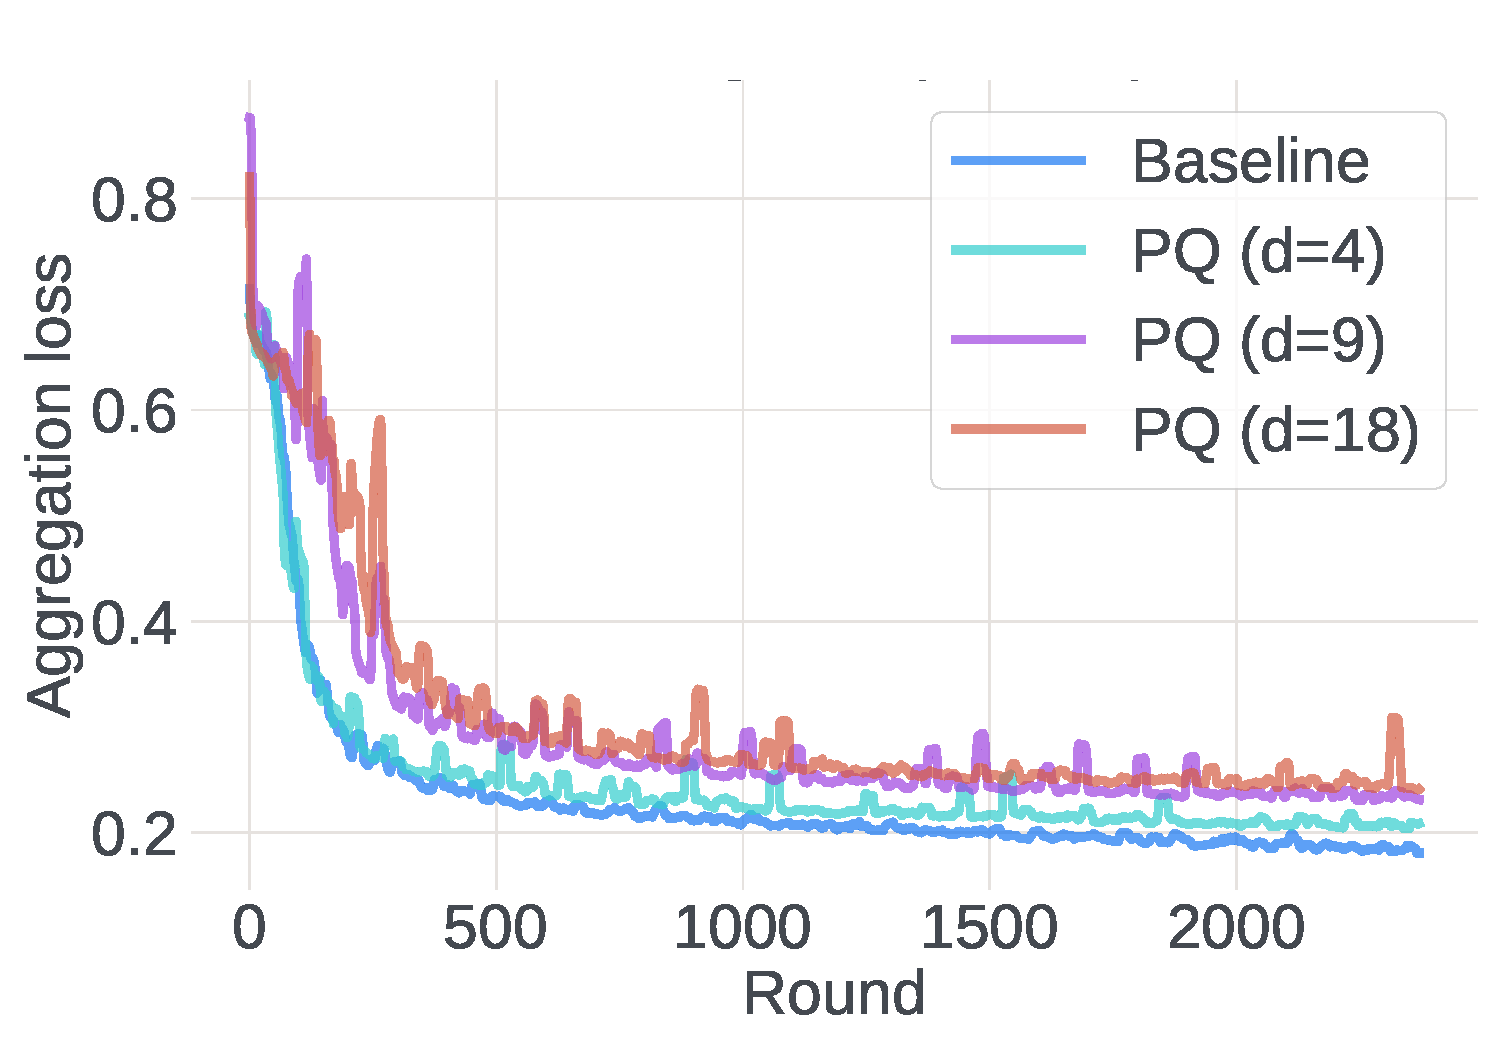
\includegraphics[width=0.6\textwidth]{submissions/GrahamCormode/figs/loss.pdf}
    \caption{\label{fig:loss}
    Number of rounds to convergence is similar for PQ-compressed runs compared to the non-compressed baseline (on CelebA).
    Note that outside a simulated environment, the wall-clock time convergence for PQ runs would be lower than the baseline since uplink communications would be faster.}
\end{figure*}

\subsubsection{Performance impact of sparsity mask refresh}
\label{sparse_refresh}

In addition to scalar and product quantization as described in Section~\ref{subsec:ablations}, we also conduct experiments with varying the interval for refreshing pruning masks. We consider two levels of sparsity, 50\% and 99\% and our experiments are on the CelebA dataset. We present our results in Figure~\ref{fig:pruning}. Overall we find that the model accuracy is robust to the update periodicity unless at very high sparsities, where accuracy decreases when mask refresh periodicity increases. This is important for future directions such as in asynchronous FL where clients have to maintain the same mask across successive global updates.
\begin{figure*}[t]
\label{fig-refresh}
    \centering
    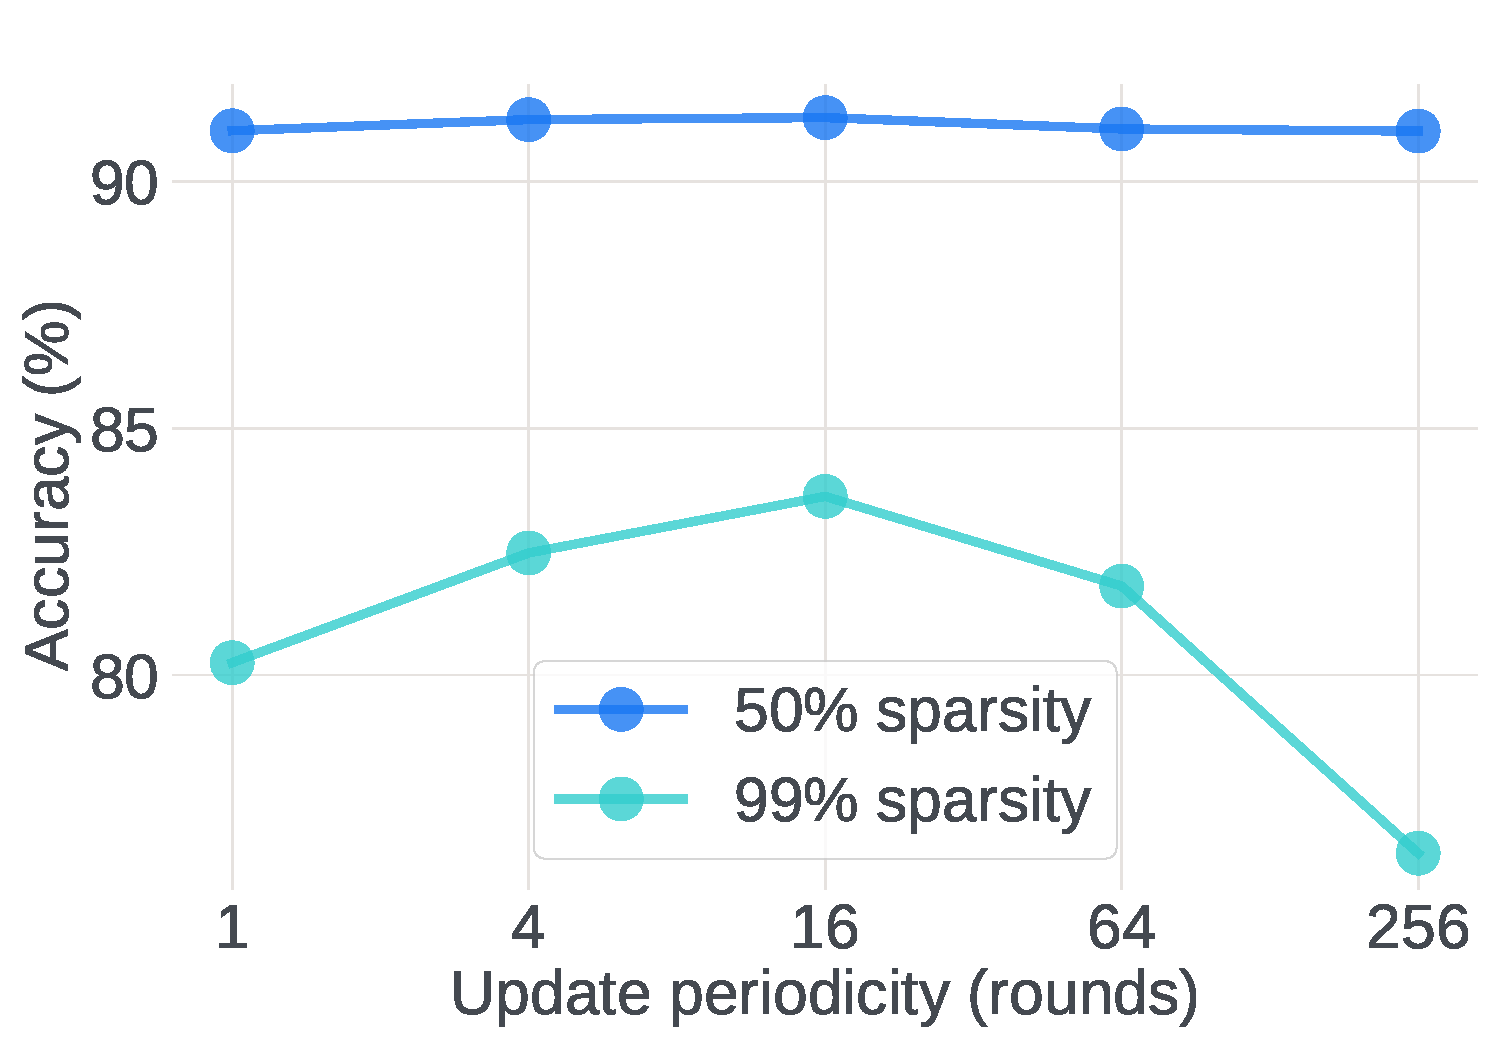
\includegraphics[width=0.5\textwidth]{submissions/GrahamCormode/figs/pruning}
    \caption{\label{fig:pruning}
    Impact of pruning mask refresh intervals on model performance for the CelebA dataset. Note that the effect of refreshing the pruning masks is more apparent at higher sparsity levels, and generalization performance decreases when masks are stale for longer during training. }
\end{figure*}


\subsection{\SecInd Implementations}
\label{appendix:secind}

\graham{
\SecInd can be implemented in other models, offering different trust paradigms.
For instance, it is natural to implement it in the multi-party computation setting
(using two or more servers to operate on shares of the input).
It would be most natural to encode the inputs as shares of one-hot vectors, but this would lose the advantages of compression.
Instead, each client can send evaluations of \emph{distributed point functions} to encode each assignment~\cite{boyle16}.
These are represented compactly, but may require longer codewords to overcome the overheads.

An advantage of working with multiple servers is that we can compute the final output (\ie the update) without exposing any intermediate representation in terms of the histogram of codewords.
That is, we could obtain shares of the histogram in the MPC model, and then use these in conjunction with the (public) codebook to build shares of the update, before finally combining these to reveal the update.
This could also be combined with the introduction of DP noise to ensure privacy as well as security.
We leave the study of such alternative implementations of \SecInd to future work.
}


\begin{table}[!ht]
\caption{Results of client update compression with \SecAgg-compatible scalar quantization on LEAF datasets over three runs. We fix $p$ across runs as this defines the uplink size, but not $b$. We pick the run with the best accuracy and report the corresponding $b$.}
    \centering
    \begin{tabular}{l|rrrrr}
    \toprule
    Dataset & $b$ & $p$ & Uplink size (in KB) & Compression factor & Accuracy \\
    \midrule
        \multirow{15}{*}{\makecell{CelebA \\ Baseline: 91.2$\pm$0.2}} & 1 & 1 & 4.3 & 26.6 & 49.3$\pm$2.7 \\
        & 1,2 & 2 & 7.9 & 14.6 & 51.8$\pm$0.4 \\
        & 2,3 & 3 & 11.4 & 10.0 & 52.0$\pm$0.7 \\
        & 1,4 & 4 & 15.0 & 7.6 & 51.8$\pm$0.5 \\
        & 3,4 & 5 & 18.5 & 6.2 & 53.9$\pm$1.7 \\
        & 1,3,5 & 6 & 22.1 & 5.2 & 52.6$\pm$0.6 \\
        & 1,2 & 7 & 25.6 & 4.5 & 52.8$\pm$1.3 \\
        & 6 & 8 & 29.2 & 3.9 & 89.6$\pm$0.2 \\
        & 6,7 & 9 & 32.7 & 3.5 & 91.2$\pm$0.1 \\
        & 6,7 & 10 & 36.3 & 3.2 & 91.2$\pm$0.3 \\
        & 6,7,8 & 11 & 39.8 & 2.9 & 91.1$\pm$0.1 \\
        & 6,8 & 12 & 43.4 & 2.6 & 91.4$\pm$0.0 \\
        & 6,7 & 13 & 46.9 & 2.4 & 91.3$\pm$0.2 \\
        & 7,8 & 14 & 50.5 & 2.3 & 91.3$\pm$0.1 \\
        & 8 & 15 & 54.0 & 2.1 & 91.2$\pm$0.2 \\
        \midrule
        \multirow{15}{*}{\makecell{Sent140 \\ Baseline: 70.8$\pm$0.4}} & 1 & 1 &  399.3 & 31.5 & 46.2$\pm$0.0 \\
        & 1 & 2 &  792.3 & 15.9 & 53.8$\pm$0.0 \\
        & 2,3 & 3 &   1185.4 & 10.6 & 53.8$\pm$0.0 \\
        & 1,2 & 4 &  1578.4  & 8.0 & 53.8$\pm$0.0 \\
        & 2,3,5 & 5 &  1971.4  & 6.4 & 53.8$\pm$0.0 \\
        & 2,6 & 6 &  2364.5  & 5.3 & 53.8$\pm$0.0 \\
        & 1,7 & 7 &  2757.5  & 4.6 & 53.8$\pm$0.0 \\
        & 2,5 & 8 &  3150.6  & 4.0 & 53.8$\pm$0.0 \\
        & 5,6,7 & 9 &  3543.6  & 3.6 & 53.9$\pm$0.0 \\
        & 4,6 & 10 &  3936.6  & 3.2 & 53.8$\pm$0.1 \\
        & 6,8 & 11 &  4329.7  & 2.9 & 53.8$\pm$0.1 \\
        & 5,7 & 12 &  4722.7  & 2.7 & 51.3$\pm$4.4 \\
        & 6,8 & 13 & 5115.7 & 2.5 & 50.6$\pm$2.9 \\
        & 7 & 14 &  5508.8  & 2.3 & 63.1$\pm$3.1 \\
        & 8 & 15 &  5901.8  & 2.1 & 68.5$\pm$1.6 \\
        \midrule
        \multirow{11}{*}{\makecell{FEMNIST \\ Baseline: 84.8$\pm$0.7}} & 1 & 1 & 1404.0 & 31.2 & 2.2$\pm$3.0 \\
        & 1,2 & 2 & 2770.3 & 15.8 & 2.4$\pm$1.5 \\
        & 3 & 3 & 4136.5 & 10.6 & 12.2$\pm$3.9 \\
        & 4 & 4 & 5502.8 & 8.0 & 65.0$\pm$3.3 \\
        & 5 & 5 & 6869.0 & 6.4 & 80.7$\pm$0.4 \\
        & 6 & 6 & 8235.3 & 5.3 & 83.8$\pm$0.2 \\
        & 5,6,7 & 7 & 9601.5 & 4.6 & 84.3$\pm$0.4 \\
        & 6,7 & 8 & 10967.8 & 4.0 & 85.1$\pm$0.1 \\
        & 6,8 & 9 & 12334.1 & 3.6 & 84.9$\pm$0.2 \\
        & 7,8 & 10 & 13700.3 & 3.2 & 85.0$\pm$0.3 \\
        & 8 & 11 & 15066.6 & 2.9 & 84.6$\pm$0.3 \\
        \bottomrule
    \end{tabular}

    \label{tab:fig2_sq}
\end{table}

\begin{table}[!ht]
    \caption{Results of client update compression  with \SecAgg-compatible random mask pruning on LEAF datasets}
    \centering
    \begin{tabular}{l|rrrr}
    \toprule
    Dataset & Sparsity & Uplink size (in KB) & Compression factor & Accuracy \\
    \midrule
        \multirow{18}{*}{\makecell{CelebA \\ Baseline: 91.2$\pm$0.2}} & 0.1 & 103.0 & 1.1 & 91.2$\pm$0.2 \\
        & 0.2 & 91.6 & 1.2 & 91.3$\pm$0.0 \\
        & 0.3 & 80.3 & 1.4 & 91.1$\pm$0.2 \\
        & 0.4 & 68.9 & 1.7 & 91.1$\pm$0.2 \\
        & 0.5 & 57.5 & 2.0 & 91.1$\pm$0.1 \\
        & 0.6 & 46.1 & 2.5 & 91.2$\pm$0.1 \\
        & 0.7 & 34.8 & 3.3 & 91.1$\pm$0.1 \\
        & 0.8 & 23.4 & 4.9 & 90.9$\pm$0.2 \\
        & 0.9 & 12.0 & 9.5 & 90.4$\pm$0.2 \\
        & 0.91 & 10.9 & 10.5 & 90.4$\pm$0.1 \\
        & 0.92 & 9.8 & 11.7 & 90.3$\pm$0.2 \\
        & 0.93 & 8.6 & 13.3 & 89.9$\pm$0.2 \\
        & 0.94 & 7.5 & 15.3 & 90.0$\pm$0.3 \\
        & 0.95 & 6.3 & 18.1 & 89.6$\pm$0.1 \\
        & 0.96 & 5.2 & 22.0 & 89.0$\pm$0.4 \\
        & 0.97 & 4.1 & 28.2 & 88.9$\pm$0.1 \\
        & 0.98 & 2.9 & 39.1 & 87.0$\pm$0.5 \\
        & 0.99 & 1.8 & 64.1 & 83.8$\pm$0.2 \\
        \midrule
        \multirow{18}{*}{\makecell{Sent140 \\ Baseline: 70.8$\pm$0.4}} & 0.1 & 11325.7 & 1.1 & 70.5$\pm$0.3 \\
        & 0.2 & 10068.0 & 1.2 & 70.6$\pm$0.5 \\
        & 0.3 & 8810.3 & 1.4 & 70.6$\pm$0.3 \\
        & 0.4 & 7552.6 & 1.7 & 70.6$\pm$1.6 \\
        & 0.5 & 6294.9 & 2.0 & 70.6$\pm$0.8 \\
        & 0.6 & 5037.1 & 2.5 & 70.3$\pm$0.9 \\
        & 0.7 & 3779.4 & 3.3 & 70.5$\pm$0.7 \\
        & 0.8 & 2521.7 & 5.0 & 67.9$\pm$0.7 \\
        & 0.9 & 1264.0 & 10.0 & 68.6$\pm$1.8 \\
        & 0.91 & 1138.2 & 11.1 & 69.4$\pm$1.1 \\
        & 0.92 & 1012.4 & 12.4 & 66.4$\pm$3.1 \\
        & 0.93 & 886.7 & 14.2 & 65.8$\pm$2.5 \\
        & 0.94 & 760.9 & 16.5 & 60.8$\pm$0.0 \\
        & 0.95 & 635.1 & 19.8 & 51.6$\pm$5.7 \\
        & 0.96 & 509.4 & 24.7 & 52.7$\pm$3.9 \\
        & 0.97 & 383.6 & 32.8 & 58.2$\pm$7.8 \\
        & 0.98 & 257.8 & 48.8 & 60.3$\pm$5.9 \\
        & 0.99 & 132.0 & 95.3 & 49.3$\pm$4.1 \\
        \midrule
        \multirow{18}{*}{\makecell{FEMNIST \\ Baseline: 84.8$\pm$0.7}} & 0.1 & 39384.2 & 1.1 & 84.6$\pm$0.3 \\
        & 0.2 & 35010.3 & 1.2 & 84.7$\pm$0.3 \\
        & 0.3 & 30636.4 & 1.4 & 84.7$\pm$0.2 \\
        & 0.4 & 26262.5 & 1.7 & 84.6$\pm$0.2 \\
        & 0.5 & 21888.5 & 2.0 & 84.3$\pm$0.3 \\
        & 0.6 & 17514.7 & 2.5 & 84.2$\pm$0.2 \\
        & 0.7 & 13140.8 & 3.3 & 83.6$\pm$0.6 \\
        & 0.8 & 8766.9 & 5.0 & 83.1$\pm$0.2 \\
        & 0.9 & 4393.0 & 10.0 & 81.7$\pm$0.4 \\
        & 0.91 & 3955.6 & 11.1 & 81.1$\pm$0.4 \\
        & 0.92 & 3518.2 & 12.4 & 80.6$\pm$0.2 \\
        & 0.93 & 3080.8 & 14.2 & 80.6$\pm$0.2 \\
        & 0.94 & 2643.4 & 16.6 & 80.2$\pm$0.3 \\
        & 0.95 & 2206.0 & 19.8 & 79.4$\pm$0.1 \\
        & 0.96 & 1768.6 & 24.7 & 78.4$\pm$0.3 \\
        & 0.97 & 1331.2 & 32.9 & 77.0$\pm$0.5 \\
        & 0.98 & 893.9 & 49.0 & 73.3$\pm$0.4 \\
        & 0.99 & 456.5 & 95.9 & 65.6$\pm$0.1 \\
        \bottomrule
    \end{tabular}

    \label{tab:fig2_prune}
\end{table}

\begin{table}[!ht]
    \centering
        \caption{Results of client update compression with Product quantization and \SecInd on LEAF datasets}
    \begin{tabular}{l|rrrrr}
    \toprule
    Dataset & $k$ & $d$ & Uplink size (in KB) & Compression factor & Accuracy \\
    \midrule
        \multirow{12}{*}{\makecell{CelebA \\ Baseline: 91.2$\pm$0.2}} & 8 & 4 & 3.4 & 33.2 & 91.0$\pm$0.2 \\
        & 8 & 9 & 1.9 & 58.9 & 89.9$\pm$0.2 \\
        & 8 & 18 & 1.4 & 83.7 & 89.1$\pm$0.4 \\
        & 16 & 4 & 4.3 & 26.3 & 91.2$\pm$0.0 \\
        & 16 & 9 & 2.3 & 49.0 & 90.7$\pm$0.0 \\
        & 16 & 18 & 1.6 & 73.0 & 89.7$\pm$0.4 \\
        & 32 & 4 & 5.2 & 21.8 & 91.4$\pm$0.1 \\
        & 32 & 9 & 2.7 & 42.2 & 90.9$\pm$0.3 \\
        & 32 & 18 & 1.8 & 65.2 & 90.1$\pm$0.1 \\
        & 64 & 4 & 6.1 & 18.7 & 91.1$\pm$0.3 \\
        & 64 & 9 & 3.1 & 37.1 & 90.9$\pm$0.1 \\
        & 64 & 18 & 1.9 & 58.9 & 90.5$\pm$0.4 \\
        \midrule
        \multirow{12}{*}{\makecell{Sent140 \\ Baseline: 70.8$\pm$0.4}} & 8 & 4 & 301.0  &   41.8   & 69.5$\pm$1.5 \\
        & 8 & 9 & 204.2  &   61.6   & 69.0$\pm$0.8 \\
        & 8 & 18 & 86.3 &    145.8   & 66.4$\pm$0.3 \\
        & 16 & 4 & 399.3  &   31.5   & 69.8$\pm$1.1 \\
        & 16 & 9 & 270.2  &   46.6   & 69.3$\pm$0.1 \\
        & 16 & 18 &  113.0 &    111.3   & 67.7$\pm$0.6 \\
        & 32 & 4 & 497.5  &   25.3   & 70.6$\pm$0.2 \\
        & 32 & 9 & 336.2  &   37.4   & 69.4$\pm$0.4 \\
        & 32 & 18 & 139.7  &   90.1   & 67.7$\pm$2.3 \\
        & 64 & 4 & 595.8  &   21.1   & 70.7$\pm$0.3 \\
        & 64 & 9 & 402.2  &   31.3   & 70.1$\pm$1.0 \\
        & 64 & 18 & 166.4  &   75.6   & 68.7$\pm$0.7 \\
        \midrule
        \multirow{12}{*}{\makecell{FEMNIST \\ Baseline: 84.8$\pm$0.7}} & 8 & 4 &   1063.3   &  41.2       & 84.4$\pm$0.4 \\
        & 8 & 9 &  494.6   &  88.5       & 82.5$\pm$0.2 \\
        & 8 & 18 &   266.4  &   164.3       & 81.5$\pm$0.4 \\
        & 16 & 4 &   1405.1   &  31.1       & 84.7$\pm$0.2 \\
        & 16 & 9 &  646.8   &  67.6       & 83.3$\pm$0.1 \\
        & 16 & 18 &   342.6  &   127.7       & 82.2$\pm$0.5 \\
        & 32 & 4 &   1747.0   &  25.0       & 84.7$\pm$0.3 \\
        & 32 & 9 &  799.1   &  54.8       & 83.9$\pm$0.6 \\
        & 32 & 18 &   418.8  &   104.5       & 83.1$\pm$0.5 \\
        & 64 & 4 &   2088.9   &  20.9       & 84.4$\pm$0.2 \\
        & 64 & 9 &  951.4   &  46.0       & 83.8$\pm$0.8 \\
        & 64 & 18 &  495.1   &  88.4       & 83.5$\pm$0.7 \\
        \bottomrule
    \end{tabular}
    \label{tab:fig2_pq}
\end{table}


\begin{table}[!ht]
    \centering
        \caption{Results of scalar quantization on LEAF datasets with unweighted client update aggregation over three runs. We fix $p$ across runs as this defines the uplink size, but not $b$. We pick the run with the best accuracy and report the corresponding $b$.}
    \begin{tabular}{l|rrrrr}
    \toprule
    Dataset & $b$ & $p$ & Uplink size (in KB) & Compression factor & Accuracy \\
    \midrule
        \multirow{15}{*}{\makecell{CelebA \\ Baseline: 91.2$\pm$0.2}} & 1 & 1 & 4.3 & 26.5 & 50.3$\pm$1.92 \\
        & 1,2 & 2 & 7.9 & 14.6 & 50.9$\pm$0.54 \\
        & 1,2,3 & 3 & 11.4 & 10.0 & 52.0$\pm$0.46 \\
        & 2,3,4 & 4 & 15.0 & 7.6 & 51.8$\pm$0.17 \\
        & 1,3,4 & 5 & 18.5 & 6.2 & 52.6$\pm$1.23 \\
        & 3,4 & 6 & 22.1 & 5.2 & 52.8$\pm$1.21 \\
        & 2,3 & 7 & 25.6 & 4.5 & 51.9$\pm$0.05 \\
        & 6 & 8 & 29.2 & 3.9 & 90.2$\pm$0.19 \\
        & 6 & 9 & 32.7 & 3.5 & 90.8$\pm$0.04 \\
        & 6 & 10 & 36.3 & 3.2 & 91.2$\pm$0.08 \\
        & 6,7 & 11 & 39.8 & 2.9 & 91.2$\pm$0.20 \\
        & 6,8 & 12 & 43.4 & 2.6 & 91.2$\pm$0.11 \\
        & 6 & 13 & 46.9 & 2.4 & 91.4$\pm$0.13 \\
        & 7,8 & 14 & 50.5 & 2.3 & 91.3$\pm$0.15 \\
        & 8 & 15 & 54.0 & 2.1 & 91.3$\pm$0.22 \\
        \midrule
        \multirow{15}{*}{\makecell{Sent140 \\ Baseline: 70.8$\pm$0.4}} & 1 & 1 & 399.3 & 31.5 & 51.3$\pm$4.4 \\
        & 1,2 & 2 & 792.3 & 15.9 & 51.3$\pm$4.4 \\
        & 1,2 & 3 & 1185.4 & 10.6 & 53.8$\pm$0.0 \\
        & 1,2 & 4 & 1578.4 & 8.0 & 53.8$\pm$0.0 \\
        & 2,3 & 5 & 1971.4 & 6.4 & 53.8$\pm$0.0 \\
        & 1,5 & 6 & 2364.5 & 5.3 & 53.8$\pm$0.0 \\
        & 1,3,4 & 7 & 2757.5 & 4.6 & 53.8$\pm$0.0 \\
        & 2,4,7 & 8 & 3150.6 & 4.0 & 53.8$\pm$0.1 \\
        & 3,5 & 9 & 3543.6 & 3.6 & 53.8$\pm$0.0 \\
        & 4,5 & 10 & 3936.6 & 3.2 & 53.8$\pm$0.1 \\
        & 5,7 & 11 & 4329.7 & 2.9 & 52.0$\pm$3.2 \\
        & 6,7 & 12 & 4722.7 & 2.7 & 53.8$\pm$0.0 \\
        & 6 & 13 & 5115.7 & 2.5 & 60.3$\pm$2.9 \\
        & 7 & 14 & 5508.8 & 2.3 & 65.9$\pm$2.9 \\
        & 8 & 15 & 5901.8 & 2.1 & 67.7$\pm$0.9 \\
        \midrule
        \multirow{11}{*}{\makecell{FEMNIST \\ Baseline: 84.8$\pm$0.7}} & 1 & 1 & 1404.0 & 31.2 & 2.0$\pm$1.3 \\
        & 1,2 & 2 & 2770.3 & 15.8 & 4.8$\pm$2.8 \\
        & 1,2,3 & 3 & 4136.5 & 10.6 & 13.6$\pm$2.4 \\
        & 4 & 4 & 5502.8 & 8.0 & 66.3$\pm$3.5 \\
        & 5 & 5 & 6869.0 & 6.4 & 79.7$\pm$0.8 \\
        & 5 & 6 & 8235.3 & 5.3 & 84.0$\pm$0.9 \\
        & 6,7 & 7 & 9601.5 & 4.6 & 84.3$\pm$0.1 \\
        & 6,7,8 & 8 & 10967.8 & 4.0 & 84.8$\pm$0.6 \\
        & 7,8 & 9 & 12334.1 & 3.5 & 85.1$\pm$0.1 \\
        & 7,8 & 10 & 13700.3 & 3.2 & 85.0$\pm$0.4 \\
        & 8 & 11 & 15066.6 & 2.9 & 83.5$\pm$1.7 \\
        \bottomrule
    \end{tabular}
    \label{tab:sq_uw}
\end{table}

